\chapter{The LHC and the ATLAS experiments} \label{chap:LHCAtlas}

The history of the European Organization for Nuclear Research (CERN) traces back to the post-WWII era, when European physicists, including Edoardo Amaldi, Niels Bohr and Pierre Auger, promoted a collaborative international laboratory dedicated to fundamental science. CERN was established in September 1954 and today it hosts the world's largest and most energetic accelerator complex, centered around the Large Hadron Collider (LHC).\\
In the following, after a description of the LHC machine, the discussion covers the architecture of the ATLAS (A Toroidal LHC ApparatuS) detector, one of the four major experiments at CERN, including its main sub-systems and simulation procedures. A special focus is given to the proton-proton collision dataset collected by ATLAS at a center-of-mass energy of 13.6 TeV during LHC Run 3, which forms the basis for this study.


%-------------------------------------------------------------------------------
%-------------------------------------------------------------------------------

\section{The LHC} \label{sec:LHCAtlas/LHC}

\begin{figure}[ht!]
    \centering
    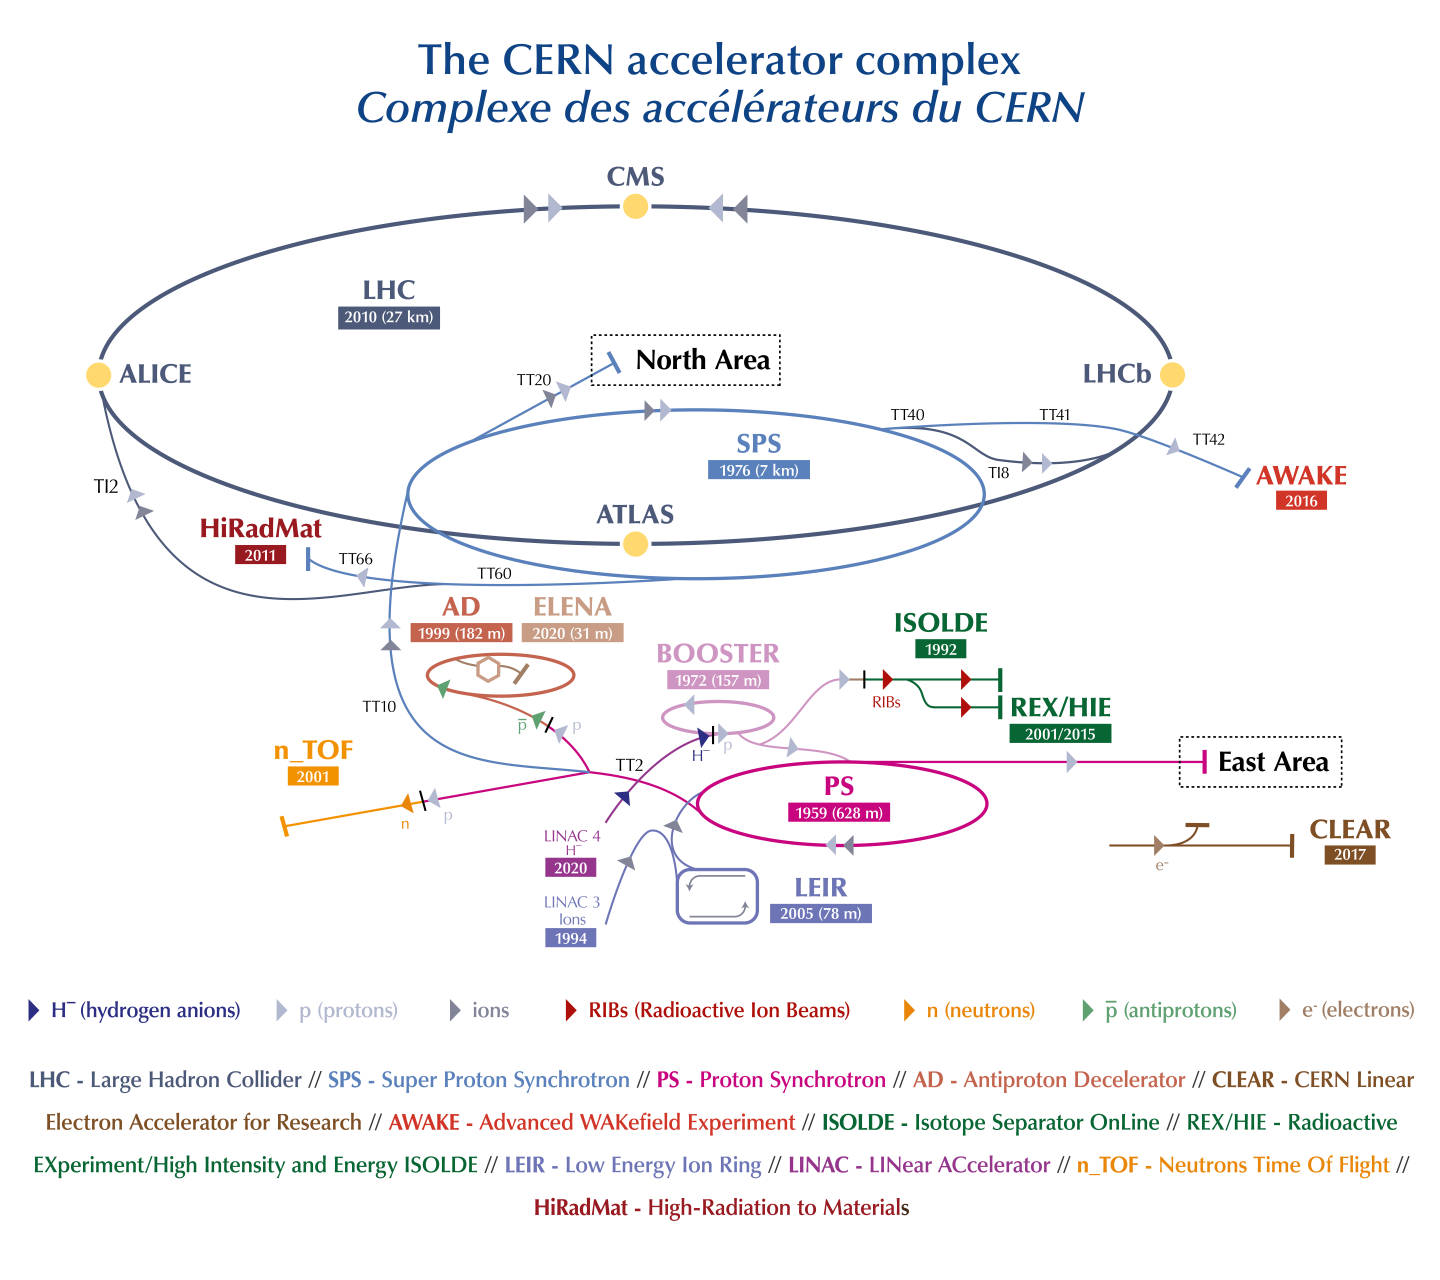
\includegraphics[width=4.5 in]{Images/Chap2/CERN_acc_system.png}
    \caption{CERN accelerating system. Figure from Ref. \cite{CERN_AcceleratorComplex}.}
    \label{fig:LHCAtlas/LHC/CERN_acc_system}
\end{figure}

The Large Hadron Collider (LHC) at CERN, with its 27 kilometres ring \cite{LHCguide}, is the world largest particle accelerator. 
It has four major interaction points which host the major CERN's experiments: ATLAS, CMS, LHCb and ALICE. 
LHC is situated around 100 metres underground to shield from radiation and for both economic\footnotemark and geological reasons. 
With its first run on 10 September 2008, it currently accelerates hadrons. Depending on the run, protons or lead nuclei are collided, with a center-of-mass energy of 13.6 TeV and 5.36 TeV respectively.
In order to reach such high energies, a complex system of pre-accelaration is adopted, as presented in Fig. \ref{fig:LHCAtlas/LHC/CERN_acc_system}.\\

\footnotetext{Building LHC on the surface would have required the purchase of properties to do so and an under the open sky structure with a 27 km circumference would have been more expensive than agreeing with landowner and excavate a tunnel underground.}


%-------------------------------------------------------------------------------

\subsection{CERN's accelerator system}\label{sec:LHCAtlas/LHC/CAS}

For proton-proton ($pp$) collisions, the process begins with the extraction of negative hydrogen ions ($H^-$), which are initially accelerated to an energy of $160\text{ MeV}$ by the Linear Accelerator 4 ($\text{LINAC4}$). 
Upon injection into the Proton Synchrotron Booster (PSB), the ions are stripped of their two electrons leaving only the bare protons, which are grouped into bunches and boosted to an energy of $2\text{ GeV}$. 
The protons then enter the Proton Synchrotron (PS), reaching an energy of $25\text{ GeV}$. 
The final step takes place in the Super Proton Synchrotron (SPS) that accelerates the proton bunches up to the LHC injection energy of $450\text{ GeV}$. 
Finally, the proton bunches are injected into the two counter-rotating beam pipes of the LHC, where they are accelerated to their maximum operational energy of $6.8\text{ TeV}$ per beam.\\
In heavy-ion operations (primarily based on lead nuclei, $^{208}\text{Pb}$), ions are initially accelerated by the Linear Accelerator 3 ($\text{LINAC3}$) to an energy of $4.2\text{ MeV per nucleon}$.
The nucleons are then accumulated and boosted to $72\text{ MeV per nucleon}$ inside the Low Energy Ion Ring (LEIR).
In the next stage, the PS accelerates ions to $5.9\text{ GeV per nucleon}$, before transferring them to the SPS where they reach an energy of $177\text{ GeV per nucleon}$. 
When injected into the main LHC ring, the heavy-ion beams are accelerated to a final energy of $2.68\text{ TeV per nucleon}$.\\
Particles are accelerated up to such high energies by means of radio-frequency (RF) cavities, resonant structures generating an oscillating electric field, with a fixed frequency of 400MHz, which accelerates charged particles each time they pass through. 
Particles with the target energy passing trough the cavity while the field is zero, will not be accelerated, while more (less) energetic particles will be decelerated (accelerated). 
Using this technique, it is ensured that particles stays in the cited bunches.


%-------------------------------------------------------------------------------

\subsection{The LHC parameters}\label{sec:LHCAtlas/LHC/parameters}

The LHC is composed by two circular beam pipes, denominated Beam 1 and Beam 2. Inside them, two particle beams, composed by a maximum of 2808 bunches with approximately $1.15\times10^{11}$ protons per bunch and spaced by 25 ns, travel separately close to the speed of light in opposite direction.
There are eight Interaction Points (IPs) along the LHC ring, but only four of them are used for collisions, hosting the main LHC experiments: ATLAS at IP1, ALICE (A Large Ion Collider Experiment) at IP2, CMS (Compact Muon Solenoid) at IP5 and LHCb (LHC beauty) at IP8.
The beam pipes and the interaction points are presented in Fig. \ref{fig:LHCAtlas/LHC/parameters/BeamsCERN}.

\begin{figure}[ht!]
    \centering
    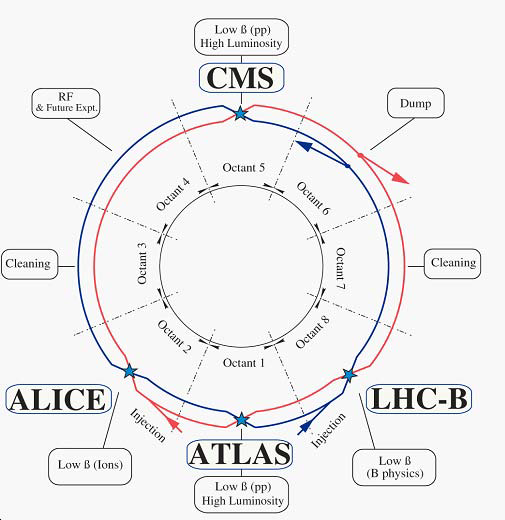
\includegraphics[width=2 in]{Images/Chap2/BeamsCERN.png}
    \caption{Schematic layout of the LHC (Beam 1 clockwise, Beam 2 anticlockwise). Figure from Ref. \cite{LHC_Machine}.}
    \label{fig:LHCAtlas/LHC/parameters/BeamsCERN}
\end{figure}

\noindent Due to the very high speed, when the two beams collide, the energy of the center of mass, known as $\sqrt{s}$, is twice the energy of each beam (which is the same). In fact, knowing that $E^2=m^2c^4+p^2c^2$ and using the natural unit system ([m]=eV/$c^2$, [p]=eV/c), we get: $E^2=m^2+p^2\simeq p^2$, where at the end an ultra-relativistic particle (p>>m) was assumed. This information is used in the norm of the four-momentum of two colliding particles:

\begin{equation}\label{eq:LHCAtlas/LHC/parameters/centerofmasseq}
    \sqrt{s}=\sqrt{P_{\mu}P^{\mu}}=\sqrt{E_{tot}^2-|\Vec{p_{tot}}|^2}=\sqrt{(E_1+E_2)^2-|\Vec{p_1}-\Vec{p_2}|^2}\simeq 2 E
\end{equation}

\noindent where we assumed $E_1$ = $E_2$. The 6.8 TeV of energy reached by LHC protons confirm the assumption p>>m and it leads to the known value of $\sqrt{s}=13.6 \text{ TeV}$.\\
Accelerated beams are directed and curved by superconducting electromagnets with a magnetic field of up to 8.3 T \cite{LHC_magnets}: 1232 dipole magnets and 392 quadrupole magnets are used to mantain the beams focused. 
Magnets are kept at a temperature of 1.9 K to ensure a 11600 A electric current which is needed for the intense magnetic field. 
Despite thier essential contribution, magnets also represent one of the main limitations of this apparatus. 
In fact, from the Lorentz force equation $\Vec{F}=q(\Vec{E}+\Vec{v}\times \Vec{B})$, it is possible to get a connection between the external magnetic field $\Vec{B}$ (the one generated by superconducting magnets), the  momentum $p$ of the particle circulating inside the beams and its radius of curvature $R$, which is:
\begin{equation}\label{eq:LHCAtlas/LHC/parameters/pqBR}
    p[GeV] = 0.3B[T]R[m]
\end{equation}

\noindent It is evident from Eq. \ref{eq:LHCAtlas/LHC/parameters/pqBR} that, to keep a constant momentum $p$ of the particles circulating inside the beams, a higher magnetic field $B$ is required in case of reduction of the radius of curvature $R$. Unfortunately, current technologies set a limit to the magnetic field generated by a magnet, limiting also the minum dimension of an accelerator ring.

\noindent Performance of the LHC are evaluated based on an essential parameter: the instantaneous luminosity $\mathcal{L}$. It defines the number of collisions per $cm^2$ and per second produced in the collider and thus it is  measured in $cm^{-2}s^{-1}$. It is computed as follows \cite{LHCreport}:
\begin{equation}\label{eq:LHCAtlas/LHC/parameters/Luminosity}
    \mathcal{L}=\frac{N_b^2n_bf_{rev}\gamma}{4 \pi \epsilon_n \beta^*}F
\end{equation}

\noindent where: $N_b$ is the number of particles in a bunch, $n_b$ is the number of bunches in a beam, $\epsilon_n$ is the normalized transverse beam emittance, $\beta^*$ is the beta function at the collision point, $\gamma$ is the Lorentz relativistic factor computed as $\gamma=1/\sqrt{1-v^2/c^2}$ , $f_{rev}$ is the revolution frequency. 
There is a connection between the beta function and the transverse beam size $\sigma$, which is $\sigma=\sqrt{\epsilon_n\beta^*/\gamma}$.
F represents the geometric luminosity reduction factor:
\begin{equation}
    F=\frac{1}{\sqrt{1+\Big(\frac{\theta_c\sigma_z}{2\sigma^*}\Big)^2}}
\end{equation}
\noindent where $\theta_c$ is the full crossing angle at the interaction point, $\sigma_z$ is the RMS bunch length and $\sigma^*$ is the transverse RMS beam size at the interaction point.
If during operations the instantaneous luminosity goes below a fixed threshold, beams are dumped and a new fill of the LHC is performed.\\
During LHC Run 3, $\mathcal{L}$ gets the value of $10^{34} \text{ cm}^{-2}s^{-1}$ for both ATLAS and CMS experiments, while for LHCb and ALICE it is $10^{32} \text{ cm}^{-2}s^{-1}$ and $10^{27} \text{ cm}^{-2}s^{-1}$ respectively.\\
The instantaneous luminosity is linked with the number of collisions per second :
\begin{equation}\label{eq:dNdt}
    \frac{dN}{dt}=\mathcal{L}\sigma_{tot}
\end{equation}
\noindent where $\sigma_{tot}$ is the total cross section, which is the measure of the probability of a specific interaction process to happen.
If the instantaneous luminosity is integrated over time, the number of events collected is obtained:
\begin{equation}\label{eq:LHCAtlas/LHC/parameters/Nevents}
    N_{events}=\sigma_{tot}\int \mathcal{L} dt 
\end{equation}

%-------------------------------------------------------------------------------

\subsection{LHC Run Schedule}

The LHC operations are structured into extended physics data-taking campaigns named \textit{Runs}, which are separated by planned technical maintenance and machine upgrade periods, which are known as Long Shutdowns (LS). 
It was Run 1, from 2010 to 2013, that started the LHC physics program, operating at center-of-mass energies of $\sqrt{s} = 7\text{ TeV}$ and $8\text{ TeV}$, with a delivered integrated luminosity of 28 $fb^{-1}$. Run 1 culminated in the discovery of the Higgs boson by the ATLAS and CMS collaborations.
Following upgrades during LS1, meant to enable higher-energy operations, Run 2 took place between 2015 and 2018 at $\sqrt{s} = 13\text{ TeV}$, delivering an integrated luminosity of approximately $156\text{ fb}^{-1}$.
After another round of upgrades during LS2 the collider entered the Run 3 era in 2022, which lasted until June 2026, operating at an increased center-of-mass energy of $\sqrt{s} = 13.6\text{ TeV}$. After having delivered an integrated luminosity of approximately $351\text{ fb}^{-1}$, the LHC was turned off for the begin of LS3.
This new stop will be used to prepare the LHC for the High-Luminosity LHC (HL-LHC) era, which is expected to start in 2029 and will last until 2042. The HL-LHC will operate at the same center-of-mass energy of Run 3 and is expected to deliver an integrated luminosity of $3000\text{ fb}^{-1}$ during the future Runs.\\
A graph showing the LHC delivered integrated luminosity during the different Runs, together with the recorded luminosity by ATLAS, is shown in Fig. \ref{fig:LHCAtlas/LHC/parameters/LumiATLAS}.

\begin{figure}[ht!]
    \centering
    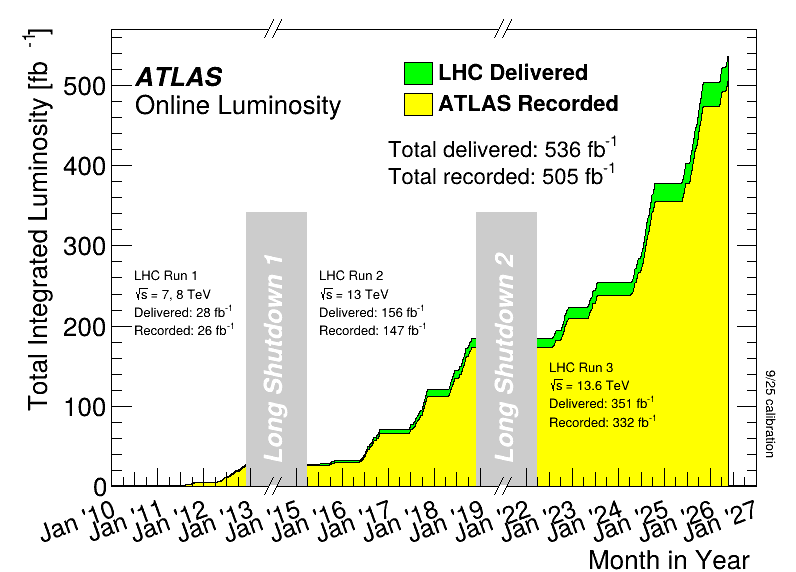
\includegraphics[width=3.5 in]{Images/Chap2/ATLAS_L_R1_R3.png}
    \caption{Cumulative integrated luminosity delivered to and recorded by the ATLAS Experiment during LHC Run 1, 2 and 3. Figure from Ref. \cite{ATLAS_Luminosity}.}
    \label{fig:LHCAtlas/LHC/parameters/LumiATLAS}
\end{figure}

%-------------------------------------------------------------------------------
%-------------------------------------------------------------------------------
\section{The ATLAS detector} \label{sec:LHCAtlas/ATLAS}

A Toroidal LHC ApparatuS (ATLAS) \cite{ATLASwebsite} is the world largest particle detector, situated at Interaction Point 1 at CERN.
44m in length and 25m in height are required to investigate collisions between particles accelerated by the LHC, to study phenomena such dark matter, the Higgs boson and top quark.
The ATLAS detector is composed by multiple sub-detectors organized in layers with a cylindrical symmetry around the beam pipe.
Among the main sub-detectors we can find: the Inner Detector (ID), the Electromagnetic Calorimeter (ECAL), the Hadronic Calorimeter (HCAL) and the Muon Spectrometer (MS), as shown in Fig. \ref{fig:LHCAtlas/ATLAS/ATLASdetector}.\\

\begin{figure}
    \centering
    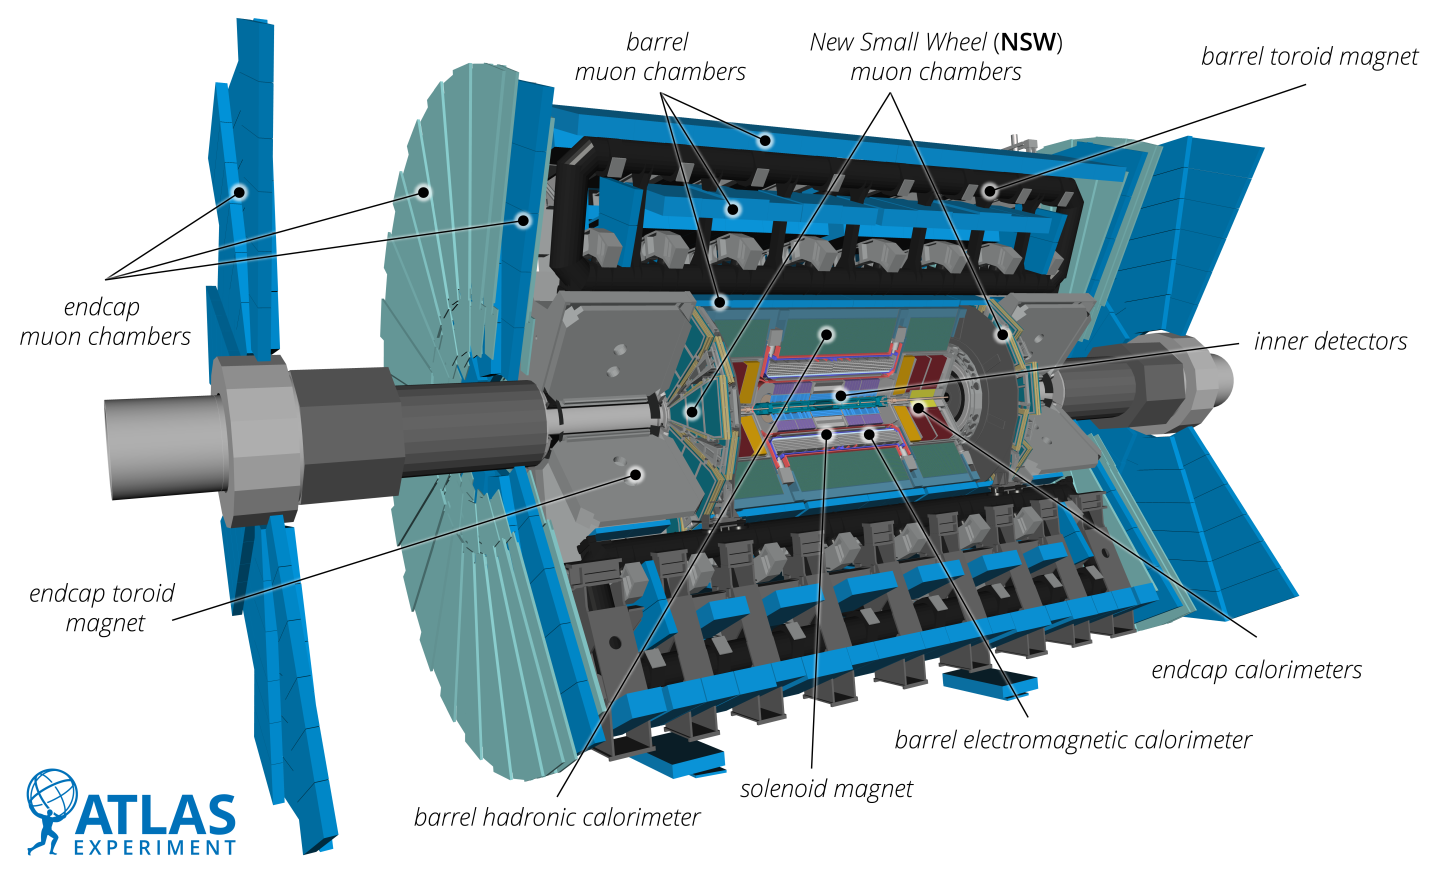
\includegraphics[width=4.3 in]{Images/Chap2/ATLASDetector.png}
    \caption{ATLAS schematic. Figure form Ref. \cite{ATLAS_detector}.}
    \label{fig:LHCAtlas/ATLAS/ATLASdetector}
\end{figure}

%-------------------------------------------------------------------------------
\subsection{Coordinate system} \label{sec:LHCAtlas/ATLAS/coordinatesystem}

Before analysing the ATLAS detector, it is important to introduce the coordinate system used to describe the position of particles and their momenta inside the sub-detectors. In figure \ref{fig:LHCAtlas/ATLAS/coordinatesystem/CoordinateSystem} an overview of the system is presented.

\begin{figure}[h!]
    \centering
    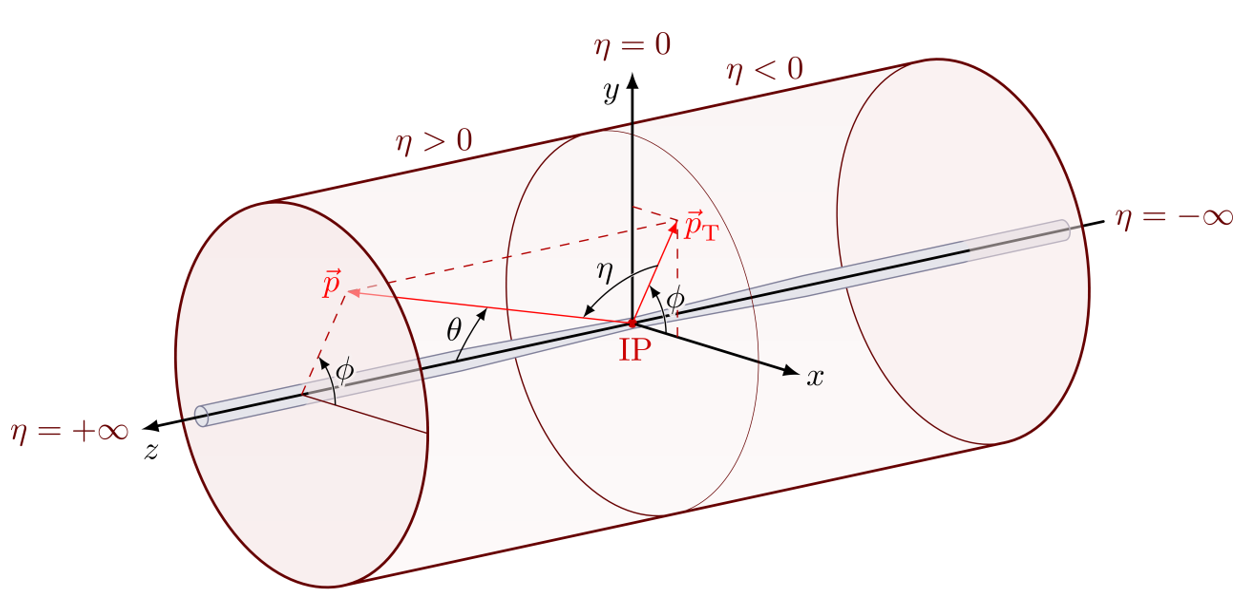
\includegraphics[width=3 in]{Images/Chap2/CoordinateSyst.png}
    \caption{Schematic of ATLAS coordinate system}
    \label{fig:LHCAtlas/ATLAS/coordinatesystem/CoordinateSystem}
\end{figure}

\noindent Cartesian axes (\textit{x,y,z}) are constructed as follows. The origin is set in the interaction point (IP). From it, the z-axis departs parallel to the beam tunnel with positive z-values in anticlockwise direction. As direct consequence, the x-y plane is perpendicular to it, with positive x-values towards the center of the LHC and positive y-values upward. On this Cartesian system, a cylindrical coordinate system ($r , \eta ,  \phi $) is defined to describe geometric position and components of particle momenta. $\phi$ is the azimuth angle, measured around the z-axis, with values [$-\pi , \pi $]. $\eta$ is named pseudo-rapidity and it is linked to the polar angle $\theta$ by the equation below:

\begin{equation}\label{eq:eta}
    \eta = - ln \Big( tan \frac{\theta}{2}\Big)
\end{equation}

\noindent The pseudo-rapidity and the azimuth angle, known as geographical coordinates \cite{ATLASexp}, are used to define a geometrical distance, applied when computing the separation between two physics objects:

\begin{equation} \label{eq:distance}
    \Delta R=\sqrt{\Delta \eta ^2 + \Delta \phi ^2}
\end{equation}

\noindent The third coordinate, $r$, is the radius from the center of the system. Actually, in this thesis, we use another information: the transverse momentum $p_T$. It is a 2D vector defined as the projection of the momentum in the transverse plane of the interaction. This parameter is related to the radius and it is important because it brings information about energy. In figure \ref{fig:pT} it is possible to observe how $p_T$ is calculated.


% \begin{figure}[h!]
%     \centering
%     \includegraphics[width=3 in]{Images/Cap4/TransverseMomentum.png}
%     \caption{Schematic of $p_T$ computing in the CMS experiment, analogous  to ATLAS}
%     \label{fig:pT}
% \end{figure}




The inner detector relies on a 2 T solenoidal magnetic field, parallel to the beam axis, to 
reconstruct the tracks of charged particles. This information is used to measure the momentum of them using the sagitta method and the relation between momentum and radius of curvature, presented in (\ref{eq:pqBR}).\\
The electromagnetic calorimeter \cite{ATLAS_detector} measures the energy of electrons, photons and hadrons. Once a particle among them hits the detector, an electromagnetic shower is generated and the energy of the particle is transferred to the material through radiation, as shown in figure \ref{fig:EMShower}. Passive components of the calorimeter such as lead induce the loss of energy and the active ones, made by Liquid Argon (LAr) kept at a temperature of -184 °C, measure it. The shower is fully contained in this part of the detector, which is longer then 20 radiation lengths. For this reason this technique to measure energy is defined \textit{destructive}.\\

% \begin{figure}[h!]
%     \centering
%     \includegraphics[width=3 in]{Images/Cap2/EMShower.png}
%     \caption{Schematic of an electromagnetic shower starting from a photon}
%     \label{fig:EMShower}
% \end{figure}

\noindent The hadronic calorimeter has been placed to measure the energy of hadrons that survive to the electromagnetic calorimeter. It relies on the principle of particle shower, which is converted into an electric current and measured.\\
The muon spectrometer is the last component of the ATLAS experiment and measures the momenta of muons. In fact, they are similar to electrons, but with a greater mass, which leads only to weak interactions and more depth of penetration. This is why they are not revealed by inner systems.\\
The coordinate system adopted at ATLAS to describe events is discussed in detail in section \ref{sec:CoordinateSystem}.
